\documentclass[a4paper,12pt]{article} % добавить leqno в [] для нумерации слева
\usepackage[a4paper,top=1.3cm,bottom=2cm,left=1.5cm,right=1.5cm,marginparwidth=0.75cm]{geometry}
%%% Работа с русским языком
\usepackage{cmap}					% поиск в PDF
\usepackage{mathtext} 				% русские буквы в фомулах
\usepackage[T2A]{fontenc}			% кодировка
\usepackage[utf8]{inputenc}			% кодировка исходного текста
\usepackage[english,russian]{babel}	% локализация и переносы

\usepackage{graphicx}
\usepackage{mathtools}
\usepackage{wrapfig}
\usepackage{tabularx}
\usepackage{amssymb}
\usepackage{hyperref}
\usepackage[rgb]{xcolor}
\hypersetup{colorlinks=true,urlcolor=blue}
%% Шрифты
\usepackage{euscript}	 % Шрифт Евклид
\usepackage{amsmath}
\usepackage{mathtools}
%%% Заголовок
\author{Lokhmatov Arseniy}
\title{Лабораторная работа по общей физике}

\date{\today}
\begin{document}
\begin{titlepage}
    \newpage
    \begin{center}
    {\large МОСКОВСКИЙ ФИЗИКО-ТЕХНИЧЕСКИЙ ИНСТИТУТ (НАЦИОНАЛЬНЫЙ ИССЛЕДОВАТЕЛЬСКИЙ УНИВЕРСИТЕТ)}
    \vspace{1cm}

    {\largeФизтех-школа аэрокосмических технологий}
    \vspace{6em}
    \end{center}
    
    \vspace{1.2em}

    \begin{center}
    %\textsc{\textbf{}}
    \Large Лабораторная работа №3.1.3 \\
    Измерение магнитного поля Земли.
    \linebreak
    \end{center}
    
    \vspace{11em}
    
    \begin{flushright}
                       {\large Работу выполнили\\
                       Лохматов Арсений Игоревич\\
                       Б03-303 }
    \end{flushright}

    \vspace{\fill}

    \begin{center}
        
\includegraphics[width=0.2\linewidth]{dasr.png}
    \end{center}

    \begin{center}
    Долгопрудный, 2024
    \end{center}

    \end{titlepage}

\section{Теоретическая часть}

\textbf{Цель работы:} исследовать свойства постоянных екодимовых магнитов; ихмерить с их помощью горизонтальную и вертикальную составляющие индукции магнитного поля Земли и магнитное наклонение.

\textbf{В работе используются:} неодимовые магниты; тонкая нить для изготовления крутильного маятника; медная проволока; электронные весы; секундомер; измеритель магнитной индукции; штангенциркуль; брусок, линейка и штатив из немагнитных материалов; набор гирь и разновесов.

\subsection*{Свойства точечного магнитного диполя}
Простейший магнитный диполь может быть образован витком с током или постоянным магнитом. По определению, магнитный момент $\overrightarrow{P_m}$ тонкого витка площадью $S$ с током $I$ равен
$$
\overrightarrow{P_m}=\dfrac{I}{c}\vec{S}=\dfrac{I}{c}S\vec{n},
$$
где $\vec{S}=S\vec{n}$ -- вектор площади круга контура. Если размеры контура с током или магнитной стрелки малы по сравнению расстоянием до диполя, то соответствующий магнитный диполь называют элементарным или точечным.\\
Магнитное поле точечного диполя определяется по формуле, аналогичной формуле для поля
элементарного электрического диполя:
$$
\vec{B}=\dfrac{3(\overrightarrow{P_m},\vec{r})\vec{r}}{r^5} - \dfrac{\overrightarrow{P_m}}{r^3}
$$ 
В магнитном поле с индукцией $B$
на точечный магнитный диполь 
действует механический
момент сил:
$$
\vec{M} = \overrightarrow{P_m}\times \vec{B}.
$$
Под действием вращающего момента $\vec{M}$ виток с током или постоянный магнит поворачивается
так, чтобы его магнитный момент выстроился вдоль вектора индукции магнитного поля. Это —
положение устойчивого равновесия: при отклонении от этого положения возникает механический
момент внешних сил, возвращающий диполь к положению равновесия. В положении, когда $\overrightarrow{P_m}$ и $\vec{B}$
параллельны, но направлены противоположно друг другу, также имеет место равновесие ($M$ = 0),
но такое равновесие неустойчиво: малейшее отклонение от этого положения приведёт к появлению
момента сил, стремящихся отклонить диполь ещё дальше от начального положения.\\
Магнитный диполь в магнитном поле обладает энергией:
$$
W = -(\overrightarrow{P_m},\vec{B})
$$
В неоднородном поле на точечный магнитный диполь, кроме момента сил, действует ещё и сила:
$$
\vec{F}=(\overrightarrow{P_m},\vec{\triangledown})\vec{B}
$$
Используя формулы для момента силы, силы и энергии, не сложно выяснить, как ведёт себя
свободный магнитный диполь в неоднородном магнитном поле: он выстраивается вдоль силовых
линий магнитного поля и, кроме того, под действием результирующей силы, возникающей из-за
неоднородности поля, втягивается в область более сильного магнитного поля, т.е. в область, где он
обладает меньшей энергией.\\
Зная магнитные моменты $P_1 = P_2 = P_m$ двух небольших постоянных магнитов, можно рассчитать силу
их взаимодействия:
$$
F = P_m \dfrac{\partial B}{\partial r}=-6\dfrac{P_m^2}{r^4}.
$$

\subsection*{Экспериментальная установка}
В настоящей работе используются неодимовые магниты шарообразной формы.
Для нас важно то, что:\\
1) шары намагничены однородно;\\
2) вещество, из которого изготовлены магниты, является магнитожёстким материалом.\\
Полный магнитный момент $\overrightarrow{P_m}$
постоянного магнита определяется намагниченностью $\overrightarrow{p_m}$
вещества, из которого он изготовлен. По определению, намагниченность – это магнитный момент единицы объёма. Для однородно намагниченного шара намагниченность равна:
$$
\overrightarrow{p_m}=\dfrac{\overrightarrow{P_m}}{V}.
$$
Намагниченность — важная характеристика вещества постоянных магнитов, определяющая, в
частности, величину остаточной магнитной индукции $B_r = 4\pi p_m$. Индукция магнитного поля $\overrightarrow{B_p}$
на полюсах однородно намагниченного шара связана с величиной намагниченности и остаточной магнитной индукцией формулами
$$
\overrightarrow{B_p}=\dfrac{8\pi}{3}\overrightarrow{p_m}=\dfrac{2}{3}\overrightarrow{B_r}.
$$

\section{Практическая часть}
\subsection{Определение магнитного момента, намагниченности и остаточной магнитной
индукции вещества магнитных шариков (метод А)}

\begin{enumerate}
    \item Взвесим шарики на весах.

    \[ m_{12} = (9.972 \pm 0.005) \text{ г.} \Longrightarrow m_{1} = (0.831 \pm 0.006) \text{ г.} \]
    
    Определим диаметр шариков.

    \begin{table}[h]
    \centering
        \begin{tabular}{|c|c|c|c|c|c|c|c|}
            \hline
            $N$ & $d$, см & $N$ & $d$, см & $N$ & $d$, см & $N$ & $d$, см \\ \hline
              1 & 0.58 & 4 & 0.60 & 7 & 0.55 & 10 & 0.55 \\ \hline
              2 & 0.59 & 5 & 0.58 & 8 & 0.60 & 11 & 0.60 \\ \hline
              3 & 0.58 & 6 & 0.60 & 9 & 0.58 & 12 & 0.58 \\ \hline
        \end{tabular}
        \label{tab1}
        \caption{Диаметр шариков}
    \end{table}

    \[ \sigma^{\text{сист}} = 0.01 \text{ см, } \sigma^{\text{случ}} = \sqrt{\frac{1}{N(N-1)}\sum_{i}^{N}(d_0 - d_{i})^2} \Longrightarrow \sigma^{\text{случ}} = 0.0051 \text{ см, } \]
    \[ \sigma = \sqrt{(\sigma^{\text{сист}})^2 + (\sigma^{\text{случ}})^2} \Longrightarrow \sigma = 0.0112 \text{ см. } \]

    \[ d = (0.5825 \pm 0.0112) \text{ см.} \]

    \item Проложите между двумя магнитными шариками брусок из немагнитного материала. Подкладывая между бруском и верхним магнитиком листы бумаги, выясните, на каком максимальном расстоянии $r_{max}$ шарики удерживают друг друга в поле тяжести Земли. 

    \[ r = (2.22 \pm 0.01) \text{ см.} \Longrightarrow r_{max} = r + d = 2.8025 \text{ см.} \]

    \item Рассчитайте величину магнитного момента магнитика $P_m$, прировняв силу притяжения двух магнитных диполей $F = 6P_m^2/r_{max}^4$ силе тяжести $F_{\text{т}} = mg$. Оцените погрешность измерений.

    \[ \frac{6P_m^2}{r_{max}^4} = mg \Longleftrightarrow P_{m} = r_{max}^2\sqrt{\frac{mg}{6}} \Longrightarrow P_m = 2.8025^2\cdot\sqrt{\frac{0.831\cdot980}{6}} = 91.502 \text{ }\frac{\text{эрг}}{\text{Гс}} \]
    \[ \sigma_{P_m} = P_m\cdot\sqrt{\left(2\cdot\frac{\sigma_{r_{max}}}{r_{max}}\right)^2 + \left(\frac{1}{2}\cdot\frac{\sigma_m}{m}\right)^2} \Longrightarrow \] 
    \[ \sigma_{P_m} = 91.502\cdot\sqrt{\left(2\cdot\frac{0.01}{2.8025}\right)^2 + \left(\frac{1}{2}\cdot\frac{0.006}{0.831}\right)^2} = 0.732 \text{ }\frac{\text{эрг}}{\text{Гс}} \]

    \item Рассчитаем величину намагниченности материала шариков.

    \[ p_m = \frac{P_m}{V}, \text{ где } V = \frac{4}{3}\pi r^3 = \frac{1}{6}\pi d^3 \Longrightarrow V = \frac{1}{6}\pi \cdot 0.5825^3 = (0.103 \pm 0.006) \text{ см}^3. \]
    \[ \Longrightarrow p_m = \frac{91.502}{0.103} = 888.37 \pm 52.24 \text{ Гс.} \]

    \item По величине магнитного момента (намагниченности) шарика, рассчитаем величину $B_p$ магнитного поля на полюсах шарика.

    \[ B_p = \frac{2P_m}{r^3} = \frac{16P_m}{d^3} \Longrightarrow B_p = \frac{16\cdot91.502}{0.5825^3} = (7.407 \pm 0.431) \text{ кГс.} \]

    \item Рассчитайте величину $B_r = 4\pi p_m$ остаточной магнитной индукции материала, из которого изготовлен магнитный шарик.

    \[ B_r = 4\cdot\pi\cdot 888.37 = (11.164 \pm 0.657) \text{ кГс.} \]

    Сравните ваш результат с табличными значениями $B_r$ для соединения неодим-железо-бор.

    \[ B_r^{table} = 12.2 \text{ кГс.} \Longrightarrow \delta = \frac{B_r^{table} - B_r}{B_r^{table}} \cdot 100\% = \frac{12.2 - 11.2}{12.2} \cdot 100\% = 8.2\%. \]
    
\end{enumerate}

\subsection{Определение магнитного момента (метод B)}

\begin{enumerate}
    \item Используя дополнительные шарики, составим цепочку из $20-30$ шариков и, с помощью неодимовых магнитов в форме параллелепипедов, подсоединим цепочку к гире и разновесам, так, чтобы общая масса системы составила $~ 500$ г. Добавляя или удаляя шарики (шарики можно примагничивать непосредственно к гире), подберём минимальный вес системы цепочки с гирей, при котором она отрывается от верхнего шарика. С помощью весов определите вес $F$ оторвавшейся цепочки с гирей.

    \[ m = (336.907 \pm 0.005) \text{ г.} \Longrightarrow F = mg = 336.907 \cdot 980 = (330.169 pm 0.005) \text{ кдин.} \]

    \item Определим силу сцепления двух шаров.

    \[ F_0 = \frac{F}{1.08} = \frac{330.169}{1.08} = (305.712 \pm 0.005) \text{ кдин.} \]

    \item Определите магнитный момент шарика $P_m$. Оцените погрешность результата.

    \[ F_0 = \frac{6P_m^2}{d^4} \Longleftrightarrow P_m = d^2\sqrt{\frac{F_0}{6}} \Longrightarrow P_m = 0.5825^2 \cdot \sqrt{\frac{305.712 \cdot 10^3}{6}} = 76.59 \text{ }\frac{\text{эрг}}{\text{Гс}} \]
    \[ \sigma_{P_m} = P_m\cdot\sqrt{\left(2\cdot\frac{\sigma_{d}}{d}\right)^2 + \left(\frac{1}{2}\cdot\frac{\sigma_{F_0}}{F_0}\right)^2} \Longrightarrow \] 
    \[ \sigma_{P_m} = 76.59\cdot\sqrt{\left(2\cdot\frac{0.0112}{0.5825}\right)^2 + \left(\frac{1}{2}\cdot\frac{0.005}{305.712}\right)^2} = 2.95 \text{ }\frac{\text{эрг}}{\text{Гс}} \]

    \item По величине магнитного момента (намагниченности) шарика, рассчитаем величину $B_p$ магнитного поля на полюсах шарика.

    \[ B_p = \frac{2P_m}{r^3} = \frac{16P_m}{d^3} \Longrightarrow B_p = \frac{16\cdot76.59}{0.5825^3} = (6.200 \pm 0.267) \text{ кГс.} \]
\end{enumerate}

\subsection{Определение магнитного момента (метод C)}

Воспользуемся магнетометром $ATE-8702$ и измерьтим индукцию поля на полюсах шарика:

\[ B_p = (4233 \pm 212) \text{Гс} \]
\[ B_p = \frac{2P_m}{r^3} = \frac{16P_m}{d^3} \Longleftrightarrow P_m = \frac{B_p\cdot d^3}{16} \Longrightarrow P_m = \frac{4233\cdot0.5825^3}{16} = 52.29 \text{ }\frac{\text{эрг}}{\text{Гс}}  \]
\[ \sigma_{P_m} = P_m\cdot\sqrt{\left(3\cdot\frac{\sigma_{d}}{d}\right)^2 + \left(\frac{\sigma_{B_p}}{B_p}\right)^2} \Longrightarrow \] 
\[ \sigma_{P_m} = 52.29\cdot\sqrt{\left(3\cdot\frac{0.0112}{0.5825}\right)^2 + \left(\frac{212}{4233}\right)^2} = 3.99 \text{ }\frac{\text{эрг}}{\text{Гс}} \]

\begin{table}[h]
\centering
    \begin{tabular}{|c|c|c|}
        \hline
        \text{ } & $P_m, \frac{\text{эрг}}{\text{Гс}}$ & $\sigma_{P_m}, \frac{\text{эрг}}{\text{Гс}}$ \\ \hline
          A & 91.502 & 0.732 \\ \hline
          B & 76.59 & 2.95 \\ \hline
          C & 52.29 & 3.99 \\ \hline
    \end{tabular}
    \label{tab2}
    \caption{Результаты вычислений}
\end{table}

\newpage

\subsection{Определение горизонтальной составляющей магнитного поля Земли}

\begin{enumerate}
    \item Соберём крутильный маятник и, используя $\Lambda$-образный подвес, установим «магнитную стрелку» из 12 магнитных шариков в горизонтальном положении (юстировка системы). 
    \item Возбудим крутильные колебания маятника вокруг вертикальной оси и определим их период. Оценим влияние упругости нити на период колебаний, возбудив крутильные колебания «стрелки», свёрнутой в кольцо.

    \[ T_{round} = (7.8 \pm 0.2) \text{ с.}, T_{line} = (3.9 \pm 0.2) \text{ с.} \]

    Видим, что период колебаний магнитной стрелки с нулевым магнитным моментом больше магнитной стрелки с ненулевым магнитным моментом. Так как период колебаний прямопропорционален $\sim \sqrt{\frac{1}{k}}$, где $k$ - коэффициент упругости, и период кольца сильно больше периода стрелки, то этот коэффициент $k$ пренебрежимо мал. Значит,  упругость нити при расчете периода
    колебаний можно не учитывать.

    \item Исследуйте зависимость периода $T$ крутильных колебаний «стрелки» от количества магнитных шариков $n$, составляющих «стрелку».

    \begin{table}[h]
    \centering
    \begin{tabular}{|c|c|c|}
        \hline
        \text{N} & $T_{10}, c$ & $T_{1}, c$ \\ \hline
          12 & 39.1 & 3.91 \\ \hline
          11 & 36.2 & 3.62 \\ \hline
          10 & 34.1 & 3.41 \\ \hline
          9 & 29.8 & 2.98 \\ \hline
          8 & 26.2 & 2.62 \\ \hline
    \end{tabular}
    \hspace{.06\textwidth}
    \begin{tabular}{|c|c|c|}
        \hline
        \text{N} & $T_{10}, c$ & $T_{1}, c$ \\ \hline
          7 & 23.5 & 2.35 \\ \hline
          6 & 20.3 & 2.03 \\ \hline
          5 & 17.1 & 1.71 \\ \hline
          4 & 15.4 & 1.54 \\ \hline
          3 & 10.1 & 1.01 \\ \hline
    \end{tabular}
    \label{tab3}
    \caption{Результаты измерений периода колебаний магнитной стрелки}
\end{table}

\item Построим график экспериментальной зависимости $T(N)$. Аппроксимируем экспериментальную зависимость $T(N)$ прямой $T=\alpha N$.

\begin{figure}[h]
    \begin{center}
		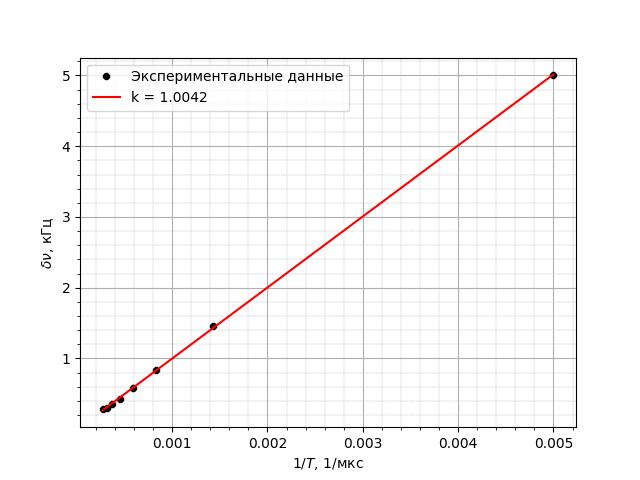
\includegraphics[width=16cm]{image2.jpg}
    \end{center}
	\caption{График экспериментальной зависимости $T(N)$}
	\label{plot4}
    \end{figure}

\item По значению углового коэффициента $\alpha$ рассчитаем величину горизонтальной составляющей магнитного поля Земли.

\[ \alpha = (0.3162 \pm 0.008) \text{ c, } B_h = \frac{\pi^2md^2}{3\alpha^2P_m}  \]
\[ \sigma_{B_h} = B_h\sqrt{\left(\frac{\sigma_m}{m}\right)^2+\left(2\frac{\sigma_d}{d}\right)^2+\left(2\frac{\sigma_{\alpha}}{\alpha}\right)^2+\left(\frac{\sigma_{P_m}}{P_m}\right)^2} \]

Рассчёты приведём для всех значений $P_m$ из таблицы \ref{tab2}.

\begin{table}[h]
\centering
    \begin{tabular}{|c|c|c|c|c|}
        \hline
        \text{ } & $P_m, \frac{\text{эрг}}{\text{Гс}}$ & $\sigma_{P_m}, \frac{\text{эрг}}{\text{Гс}}$ & $B_h, \text{Гс}$ & $\sigma_{B_h}, \text{Гс}$ \\ \hline
            A & 91.502 & 0.732 & 0.101 & 0.007 \\ \hline
            B & 76.59 & 2.95 & 0.121 & 0.009 \\ \hline
            C & 52.29 & 3.99 & 0.177 & 0.018 \\ \hline
    \end{tabular}
    \label{tab4}
    \caption{Результаты вычислений}
\end{table}    
\end{enumerate}

\subsection{Определение вертикальной составляющей магнитного поля Земли}

\begin{enumerate}
    \item Изготовим магнитную «стрелку» из $n = 10$ шариков и подвесим её за середину с помощью нити на штативе.
    \item Определим механический момент сил, действующий со стороны магнитного поля Земли на горизонтально расположенную магнитную «стрелку».

    \[ M = m_{\text{гр}}gl \text{,    } \sigma_M = M\sqrt{\left(\frac{\sigma_l}{l}\right)^2+\left(\frac{\sigma_m}{m}\right)^2} \text{, где } \sigma_l = 0.1 \text{ см, } \sigma_m = 0.005 \text{ г} \]
    
    Для этого, с помощью одного или нескольких кусочков проволоки, уравновесим «стрелку» в горизонтальном положении. С помощью весов определим массу уравновешивающего груза $m_{\text{гр}}$. Из условия равновесия рассчитаем механический
    момент сил $M$, действующих на горизонтальную «стрелку» со стороны поля Земли для нескольких значений $n$. Результаты занесём в таблицу \ref{tab5}.

    \begin{table}[h]
    \centering
    \begin{tabular}{|c|c|c|c|c|c|}
        \hline
        n, \text{ шт} & 12 & 10 & 8 & 6 & 4 \\ \hline
            $m_{\text{гр}}, \text{ г}$ & 0.173 & 0.197 & 0.221 & 0.263 & 0.352 \\ \hline
            $l, \text{ см}$ & 3.45 & 2.76 & 2.07 & 1.38 & 0.69 \\ \hline
            $M, \text{ дин см}$ & 584.913 & 532.846 & 448.321 & 355.681 & 238.022 \\ \hline
            $\sigma_M, \text{ дин см}$ & 23.942 & 23.572 & 23.916 & 26.646 & 34.661 \\ \hline
    \end{tabular}
    \label{tab5}
    \caption{Результаты измерений момента сил}
\end{table}

\item Постройте график экспериментальной зависимости $M=M(n)$. Аппроксимируйте экспериментальную зависимость $M(n)$ прямой линией $M=\beta n$.

Нагляно видно, что с увеличением числа шариков (увеличение магнитного момента) увеличивается механический момент сил. 

\begin{figure}[h]
    \begin{center}
		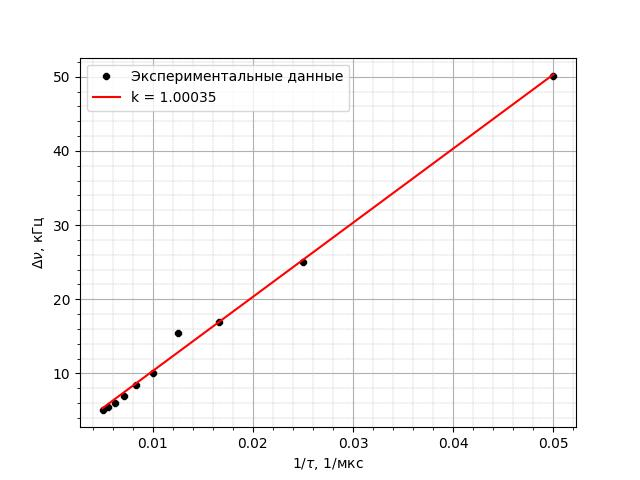
\includegraphics[width=16cm]{image1.jpg}
    \end{center}
	\caption{График экспериментальной зависимости $M(n)$}
	\label{plot4}
    \end{figure}

\itemПо значению углового коэффициента $\beta$ зависимости $M = \beta n$ рассчитаем величину $B_v$ вертикальной составляющей магнитного поля Земли.
Оцените погрешность измерений $B_v$.

\[ \beta = (43.547 \pm 3.435) \text{ дин см} \]
\[ \beta = B_v P_m \Longleftrightarrow B_v = \frac{\beta}{P_m} \text{, } \sigma_{B_v} = B_v\sqrt{\left(\frac{\sigma_{\beta}}{\beta}\right)^2 + \left(\frac{\sigma_{P_m}}{P_m}\right)^2} \]

Рассчёты проведём для всех $P_m$, полученных ранее. Результаты занесём в таблицу \ref{tab6}.

\begin{table}[h]
\centering
    \begin{tabular}{|c|c|c|c|c|}
        \hline
        \text{ } & $P_m, \frac{\text{эрг}}{\text{Гс}}$ & $\sigma_{P_m}, \frac{\text{эрг}}{\text{Гс}}$ & $B_v, \text{Гс}$ & $\sigma_{B_v}, \text{Гс}$ \\ \hline
            A & 91.502 & 0.732 & 0.476 & 0.038 \\ \hline
            B & 76.59 & 2.95 & 0.569 & 0.05 \\ \hline
            C & 52.29 & 3.99 & 0.833 & 0.091 \\ \hline
    \end{tabular}
    \label{tab6}
    \caption{Результаты вычислений}
\end{table}  

\item Используя результаты измерений $B_h$ и $B_v$, определите магнитное наклонения $\gamma$ и полную величину индукции магнитного поля Земли на широте Долгопрудного. Сравните полученное значение наклонения с расчётным, полученным в предположении, что магнитное поле Земли соответствует полю однородно намагниченного вдоль оси вращения шара. Оцените также полный магнитный момент $P_3$ Земли.

\[ \gamma = \arctan{\frac{B_v}{B_h}} \text{, } B = \sqrt{B_v^2 + B_h^2} \text{, } \sigma_B = \sqrt{\sigma_{B_v}^2 + \sigma_{B_h}^2} \]
\[ B_{table} = 0.4 \text{ Гс} \]
    
\end{enumerate}

\section{Подведение итогов и выводы}

В данной работе мы измерили магнитный момент неодимовых шарообразных магнитов тремя разными способами, и, зная этот момент, рассчитали вертикальную и горизонтальную составляющие магнитного поля Земли, а так же полную магнитную индукцию поля Земли. Результаты представлены в таблице \ref{tab7}. 

\begin{table}[h]
\centering
    \begin{tabular}{|c|c|c|c|c|c|c|c|c|c|}
        \hline
        \text{ } & $P_m, \frac{\text{эрг}}{\text{Гс}}$ & $\sigma_{P_m}, \frac{\text{эрг}}{\text{Гс}}$ & $B_h, \text{Гс}$ & $\sigma_{B_h}, \text{Гс}$ & $B_v, \text{Гс}$ & $\sigma_{B_v}, \text{Гс}$ & $\gamma \text{, град}$ & $B, \text{Гс}$ & $\sigma_B, \text{Гс}$ \\ \hline
            A & 91.502 & 0.732 & 0.101 & 0.007 & 0.476 & 0.038 & 77.973 & 0.487 & 0.038 \\ \hline
            B & 76.59 & 2.95 & 0.121 & 0.009 & 0.569 & 0.05 & 77.973 & 0.581 & 0.051 \\ \hline
            C & 52.29 & 3.99 & 0.177 & 0.018 & 0.833 & 0.091 & 77.973 & 0.851 & 0.093 \\ \hline
    \end{tabular}
    \label{tab7}
    \caption{Результаты вычислений}
\end{table}

Ближе всего к табличному значению оказалось значение, полученное с помощью метода А.

Неточность измерений в других методах может быть связана с неточными методами измерения такие как измерение периода колебаний магнитной стрелки (не исключено, что срелка поворачивалась не в одной плоскости). Так же другие магнитные поля в лаборатории могли вносить добавку в полученные значения.


\end{document}
